\subsection{Archetype variations across Gender}
\label{sec:discussion}
We now proceed to analyze the variations in the evolution of research interests (or archetypes) between male and female researchers. To this end, we manually annotate gender of all current and emeritus professors in top 50 Computer Science (CS) Universities as reported by U.S. News \& World Report\footnote{\url{bit.ly/usnews-cs}}. We consider only current and emeritus \emph{Full} Professors as they typically have 15 or more years of publication history. This results in a total of 1084 authors in our dataset, 127 of whom are women. ~\Cref{tab:acadclusterdata} shows the distribution across archetypes. We observe similar gender distribution in each archetype with the least number of women academics in \emph{evolving} archetype.

\begin{table}[h]
    \centering
    \begin{tabular}{l r r r r}
        \toprule
             Social Group   & Steady  & Diverse & Evolving & Diffuse \\ \midrule
        Male    Professors (Top-50 US schools) & 247     & 206     & 241    & 263   \\
        Female Professors (Top-50 US schools) & 30     & 32    & 26    & 39  \\
        All authors in the dataset   & 1329    & 1080     & 1107    & 1062   \\ \bottomrule %
    \end{tabular}
    \caption{ \label{tab:acadclusterdata} Statistics for discovered archetypes in relationship to different social groups.}
\end{table}


While researchers from both genders in the same archetype $c$ will traverse the same set of stages, they may differ in \textit{how} they transition $\tau^c$, and at \textit{which} stage they start $\pi^c$. For this analysis, we first run our model on the entire dataset assigning archetypes to each individual. We then estimate separate model parameters for female $\lambda^c_f$ and male $\lambda^c_m$ researchers for each archetype $c$ using the assigned values.

To quantify the difference between two models ($\lambda^c_f, \lambda^c_m$) for archetype $c$, we compute their \emph{likelihood ratio}. Likelihood ratio $R^c_f$ of female researchers in archetype $c$ is:

\begin{equation}
    R^c_f = \exp \left ( \frac{1}{|N^c_f|} {\sum_{i \in {N_f}} \log \frac{ P(X_i | \lambda_f^c)}  {P(X_i | \lambda_m^c)}} \right )
    \label{eq:confusion metric}
\end{equation}

where $N^c_f$ represents all female researchers in $c$-th archetype. The equation simplifies to say that $\displaystyle \log R^c_f$ is the average difference between log-likelihoods of a trajectory of a female researcher generated from their own model with those of male model of the same archetype. Thus, for instance, value of $\displaystyle R^c_f = 2$ denotes that female researchers are twice more likely to be generated by the model of their own gender than of the opposite gender. We compute a similar ratio, $R^c_m$, for men. We also conduct paired-sample t-test \cite{goulden:1949} between the two likelihood values similar to ~\Cref{sec:acad}.

\begin{table}[tbh]
    \centering
    \begin{tabular}{lllll}
        \toprule %
        Gender & Steady & Diverse & Evolving & {Diffuse} \\
        \midrule
        Male   & 2.10***  & 2.63**  & 1.15  & 1.10   \\
        Female & 1.80***  & 1.64**  & 1.60***  & 1.38***    \\
        \bottomrule
    \end{tabular}
    \caption{
    \label{tab:genderclusterdata} Likelihood ratio for academics across genders within an archetype. It measures odds of a researcher being better explained by model for their gender than by model for the other gender.\\ $* = p < .05, ** = p< .01, *{*}* = p < .001$}
\end{table}

\Cref{tab:genderclusterdata} shows the likelihood ratio with their $p$-values. Since most of the values are statistically significant, all researchers are better explained by the model for their gender, than by the model for the opposite gender. Male researchers are distinct for the steady and diverse archetypes, but not for the evolving and diffuse archetypes. For women, on average, the difference is larger, with the strongest difference seen for the steady, diverse, and evolving archetypes.

\begin{figure*}[tbh]
        \centering
        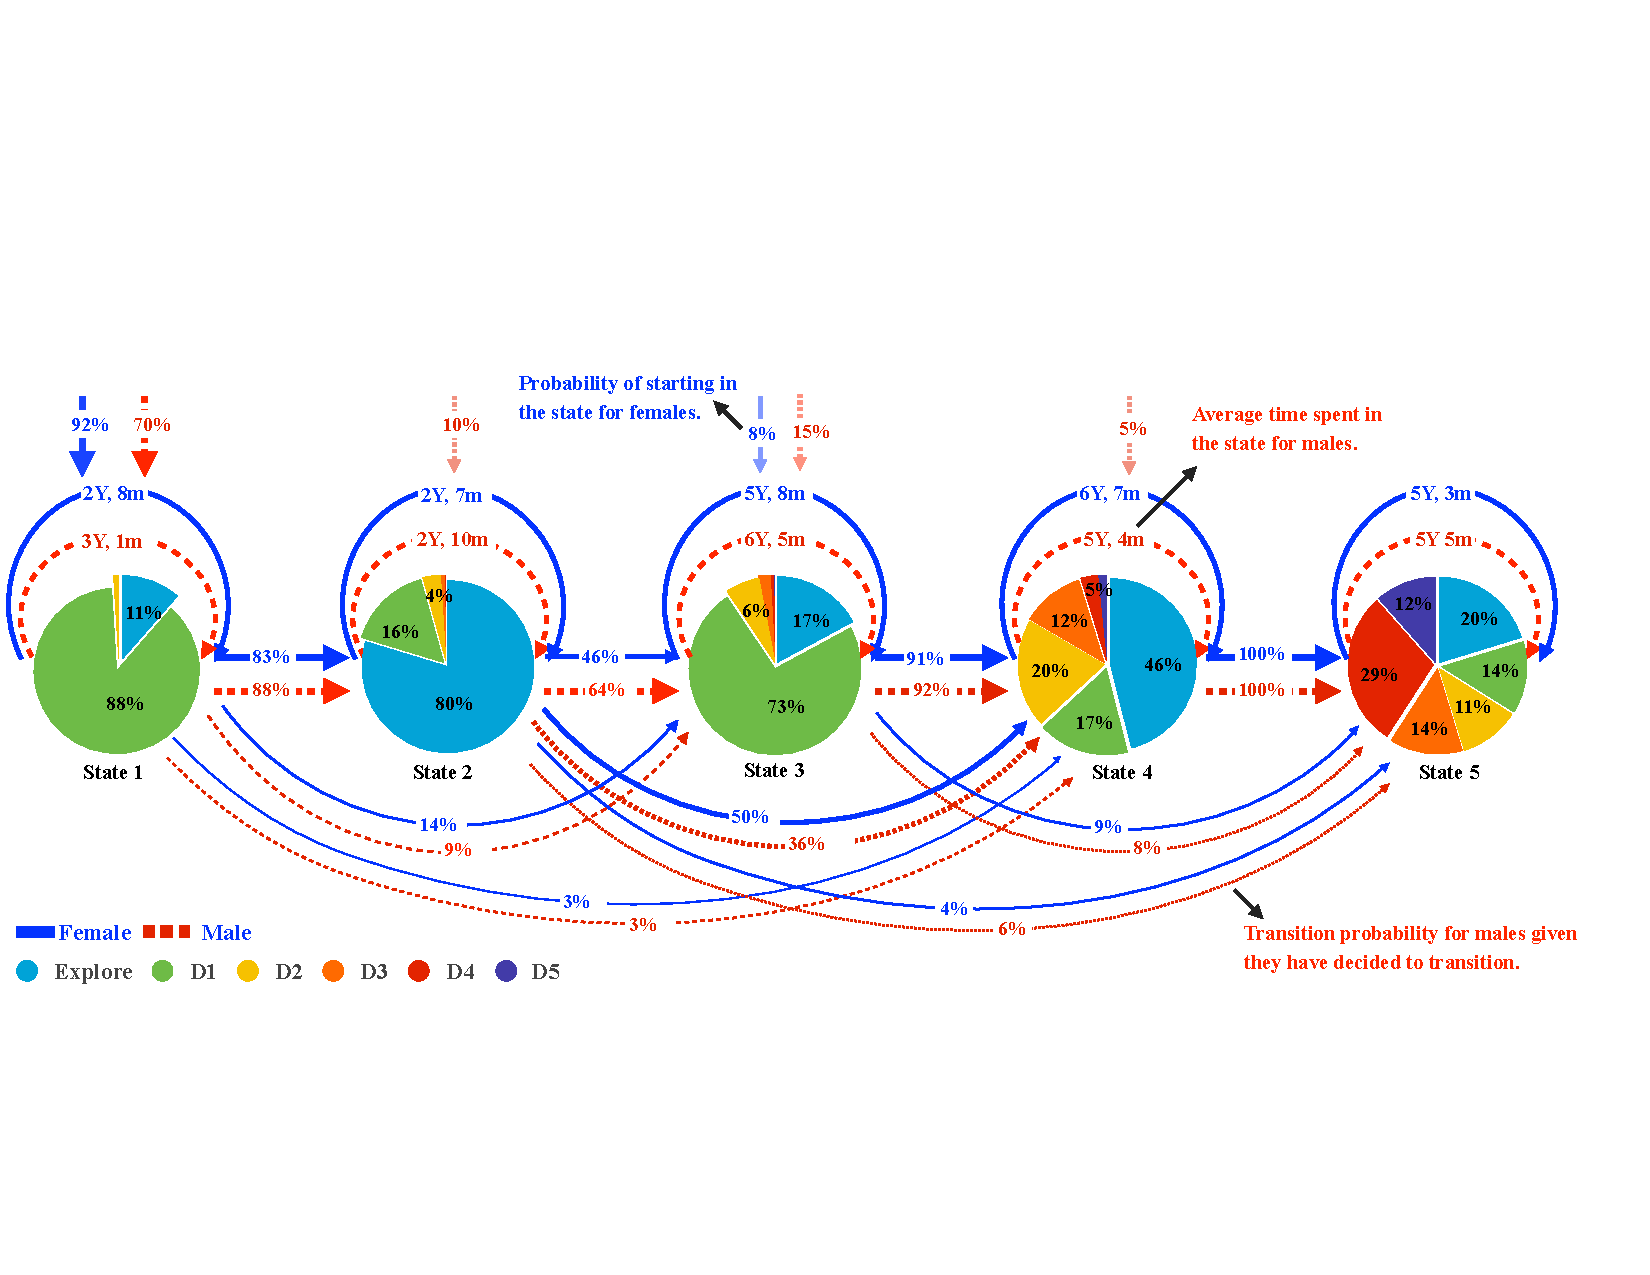
\includegraphics[width=1\linewidth,height=7cm]{figures/Cluster3_both_Self.pdf}
    \caption{
    \label{fig:genderacadclusters} Gender wise representation of trajectory for researchers belonging to the \emph{diverse} archetype in the Academic Dataset. The transitions in blue denote transition probabilities of female professors in the archetype while those in red represents probabilities for their male counterparts. Men start their career from later evolved stages while women make long term state transitions.}
    \label{fig:academic_gender}
\end{figure*}

For the sake of brevity, we examine gender difference in only the \emph{diverse} archetype in some detail. ~\Cref{fig:academic_gender} shows three interesting variations. First, we observe that women are much more likely to start in state 1 (92\%), with a dominant area of interest ($D_1$) than in any other state. In contrast, men start in states 1, 2, 3, and 4, with only 70\% starting in state 1. Both men and women skip stages, but women are more likely to skip a stage than men. For example, 50\% of women skip stage 3, while only 36\% of men do. Longer skips of two stages are rarer, and both women and men make these long skips at the same rate. Finally, there are clear differences between mid-career men and women (states 3, 4): women spend more time \emph{exploring} mid-career (state 4) than men, and mid-career men spend more time in their starting area of interest ($D_1$, state 3) than women.

\subsection{Grant income variability across Archetypes \& gender within an Archetype}
\label{sec:grant}
We next examine the relationship between variation in the academic trajectories and gender to research grants awarded at different stages of an academic career. We extract historical information of grants from the National Science Foundation, a large federal funding agency for Science \& Engineering in the United States \footnote{\url{bit.ly/nsfgrants}}. We consider grants with Principal Investigators (PI) from the same subset of CS professors in top-50 US universities as in~\Cref{sec:discussion}. We collect information for 1062 professors and manually disambiguate names and identify gender by cross-validating with the researcher's webpage.
Then, we compute the average grant money awarded to a researcher, at each stage in their trajectory. ~\Cref{fig:grantanalysis}, which shows letter-value plots of average grant size awarded as PI's, broken down by archetypes (steady, diverse, evolving or diffuse), stage within an archetype and gender, summarizes our findings.

\begin{figure*}[tbh]
    \centering
    \begin{subfigure}{0.5\linewidth}
        \centering
        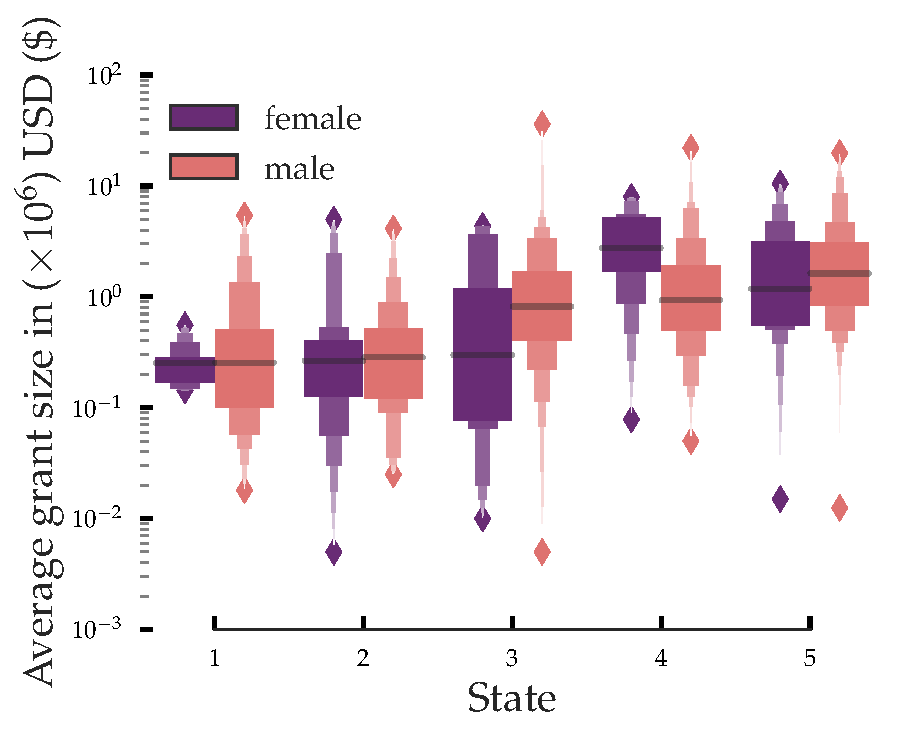
\includegraphics[width=0.8\linewidth,height=5cm]{figures/Cluster_4_PI_grant.pdf}
        \caption{Steady Researchers}
    \end{subfigure}%
    \begin{subfigure}{0.5\linewidth}
        \centering
        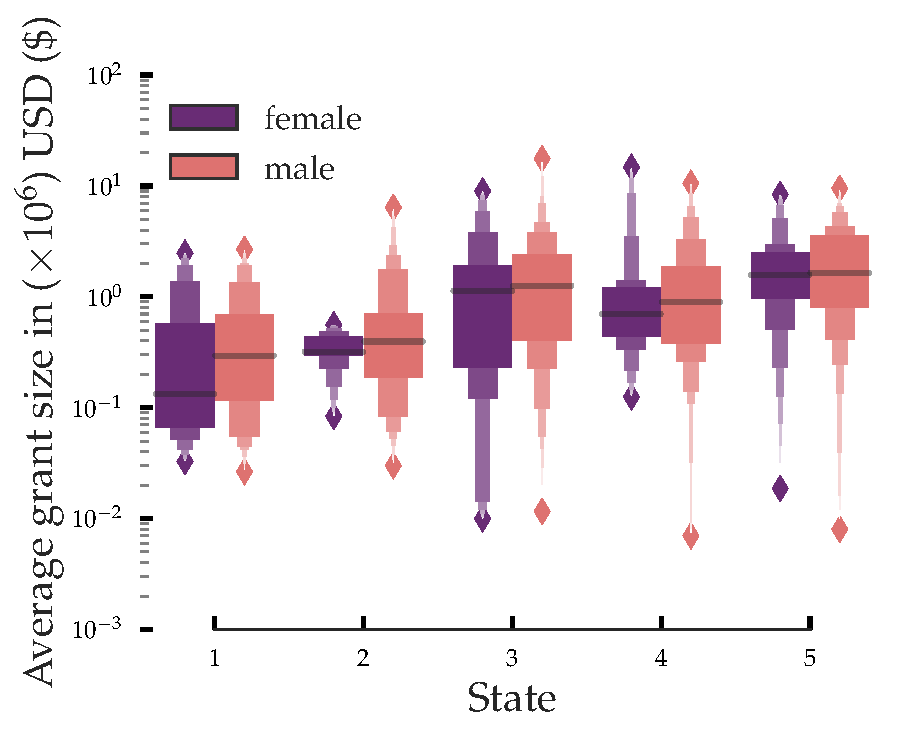
\includegraphics[width=0.8\linewidth,height=5cm]{figures/Cluster_3_PI_grant.pdf}
        \caption{Diverse Researchers}
    \end{subfigure}
    \begin{subfigure}{0.5\textwidth}
        \centering
        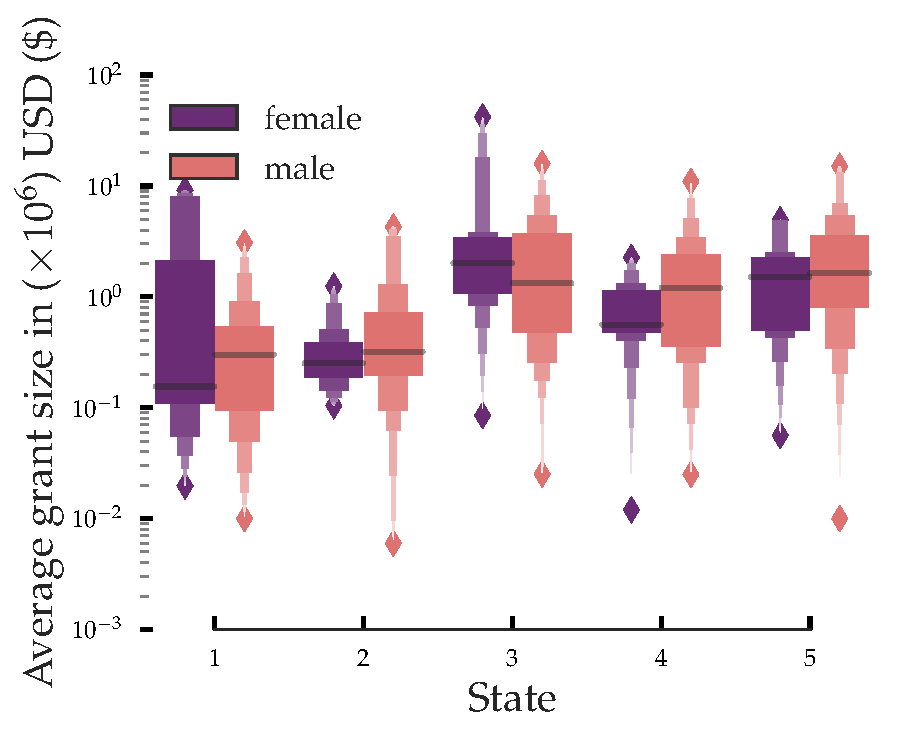
\includegraphics[width=0.8\linewidth,height=5cm]{figures/Cluster_1_PI_grant.pdf}
        \caption{Evolving Researchers}
    \end{subfigure}%
    \begin{subfigure}{0.5\textwidth}
        \centering
        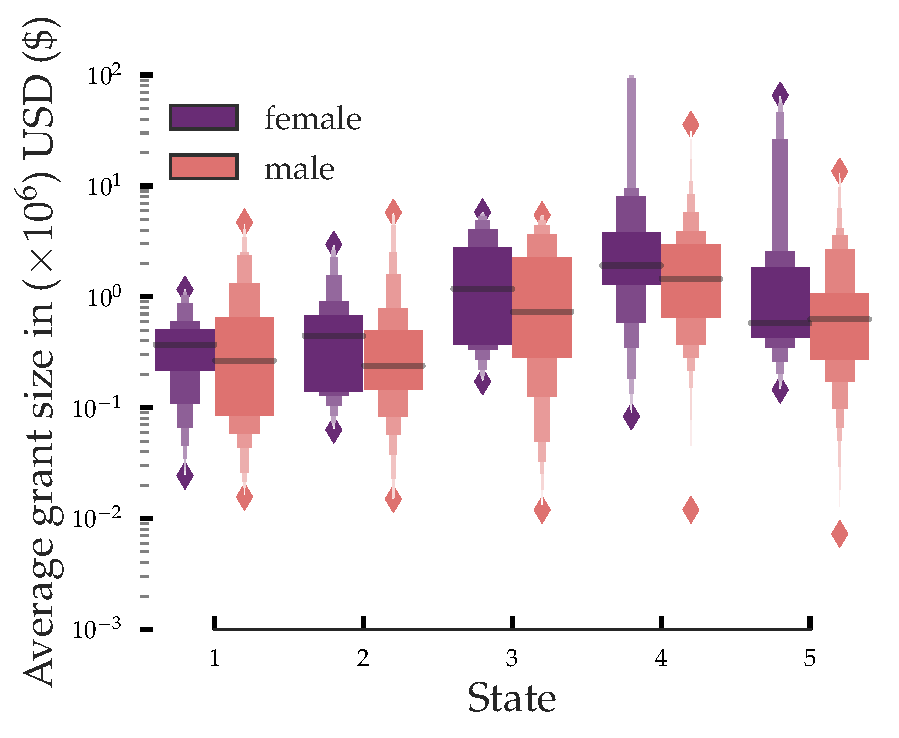
\includegraphics[width=0.8\linewidth,height=5cm]{figures/Cluster_2_PI_grant.pdf}
        \caption{Diffusive Researchers}
    \end{subfigure}
    \caption{\small \label{fig:grantanalysis} Letter value plots of total grant money awarded by NSF when author is a PI in each stage. In general, Professors get more grant money as they gain experience. Regardless of archetypes, grant income in state 3 is significantly higher from state 2 (p< .01). There are also significant differences across genders within a state of an archetype. For instance, for Evolving archetype, male professors get significantly more income than female professors in state 4 (p < .01).}
\end{figure*}

\begin{table}[tbh]
\centering
\begin{tabular}{ll}
\toprule
Archetype (H-test) &  State Pair (t-test)  \\
\midrule
\multirow{2}{*}{Steady***}    & State 2 vs 3**    \\
                     & State 4 vs 5*    \\
\hline
\multirow{2}{*}{Diverse***}   & State 2 vs 3*** \\
                                    & State 4 vs 5*    \\ \hline
\multirow{3}{*}{Evolving***}  & State 2 vs 3***   \\
                         & State 3 vs 4*    \\
                        & State 4 vs 5**    \\ \hline
\multirow{1}{*}{Diffuse***}   & State 2 vs 3***     \\
\bottomrule
\end{tabular}
\caption{ \small Statistical significance tests for the differences in grant money across latent states within an archetype. Shown are only those tests that are statistically significant. H-test \cite{Kruskal:1952} confirms that at least one state is different from another state of the archetype; t-test \cite{Welch:1947} was then conducted between each consecutive states within the archetype to determine the differing states. $* = p < .1, ** = p< .01, *{*}* = p < .001$ }
\label{tab:statstate}
\end{table}


Additionally, we conducted Kruskal-Wallis H-test~\cite{Kruskal:1952} to establish the statistical significance of differences in grant money across latent states within an archetype. This test affirms that at least one latent state is different from another latent state within an archetype \footnote{ We also conducted H-test for the difference in average grant income across archetypes for the same state. However, we did not find any significant differences. \Cref{fig:grantanalysis} can easily verify this lack of difference. }. We then conducted Welch's t-test~\cite{Welch:1947} between consecutive states to find the exact pair of states which are significantly different. We only tested with consecutive latent states as we are only interested in grant income changes as the author progresses through stages. ~\Cref{tab:statstate} reports the state pairs for each archetype that are statistically different. In the rest of this section, we describe these results in detail.

Regardless of archetypes, we observe that in general authors tend to receive more grant money as they gain experience in~\Cref{fig:grantanalysis}. On average, across archetypes and gender, PI's receive in state 5, four times the amount of grant money than state 1 ($p < .001$). Also for researchers across archetypes and across genders, we notice an uptick in grant income in state 3 from state 2 ($p < .01$ - ~\Cref{tab:statstate}). Let us qualitatively examine the \emph{steady} researchers in detail, by comparing~\Cref{fig:grantanalysis} with~\Cref{fig:acadclusters}. State 2 in~\Cref{fig:acadclusters} shows the researchers exploring different topics, whereas, in state 3, they are spending a significant part of their time on their main domain $D_1$. Also, notice that 36\% of the researchers never visit state 2 - 27\% skip state 2, and 9\% of the researchers start in state 3. Since state 1 typically represents the time spent by the researchers in their Ph.D., and with 74\% time spent in an explore stage in state 2, it is not surprising that we see limited grant income in their first two states. State 3, perhaps reflects a sustained focus on their domain $D_1$, and this pays off in terms of grant income. Similar qualitative arguments follow for the other archetypes.


\begin{table}%[tbh]
\centering
\begin{tabular}{ll}
\toprule
Archetype & Latent State (t-test) \\
\midrule
\multirow{2}{*}{Steady}   & State 1* \\
& State 4*  \\ \hline
Diverse   &  State 2*  \\ \hline
\multirow{2}{*}{Evolving}  & State 4** \\
& State 5*    \\  \hline
Diffuse & {Not significant}  \\
\bottomrule %\hline
\end{tabular}
\caption{ \small
\label{tab:statgender}Statistical significance tests \cite{Welch:1947} for the differences in grant money across gender in each state within an archetype. Shown are only those tests that are statistically significant. \\ $* = p < .1, ** = p< .05, *{*}* = p < .001$}
\end{table}

However, the grant trajectories over states is different for each archetype ($p < .001$). Let us examine statistically different state pairs from ~\Cref{tab:statstate} in ~\Cref{fig:grantanalysis}. Steady researchers see a big uptick in their grant income in state 3 ($p < .01$) and a dip in state 5 ($p < .1$), perhaps due to switching back to their primary research area. The grant income for diverse researchers (who have more than one dominant area) increases steadily over states($p < .05$). For evolving researchers (who change their dominant area), the grant income rises (state 3, $p < .001$), falls (state 4, $p < .05$) and rises (state 5, $p < .1$), reflecting a degree of unpredictability accompanying \emph{changing area of interest}. Diffuse researchers see an increase in funding in state 3 ($p < .001$) with similar grant income in subsequent states.

To determine differences in grant income across gender, we further conducted t-test \cite{Welch:1947} between grant distributions of female and male professors in each state within an archetype. ~\Cref{tab:statgender} reports significantly different states within each archetype. We again examine these statistically different states from ~\Cref{tab:statgender} in ~\Cref{fig:grantanalysis}. Evolving women receive significantly \emph{lower} income than evolving men when they \emph{switch to new areas} in state 4 and 5 ($p < .05$). On the other hand, in our dataset, steady women receive significantly \emph{higher} grant income than steady men when they \emph{switch areas} in state 4 ($p < .05$). In general, we observe that men show greater grant income variability than do women. The variability is statistically significant ($p < .05$) during early career in state 1 and 2 for Steady and Diverse researchers respectively. We do not observe significant differences in grant income of male and female Diffusive researchers.
